\documentclass[UTF8,AutoFakeBold]{ctexart}

\usepackage[]{color}

\usepackage{graphicx}  %插入图片的宏包
\usepackage{float}     %设置图片浮动位置的宏包
\usepackage{subfigure} %插入多图时用子图显示的宏包
\usepackage{listingsutf8}   %代码

\usepackage{geometry}  %设置边距
\usepackage{verbatim}  %显示原始字符
\usepackage{cprotect}  % 在标题中显示原始字符
\usepackage[colorlinks=true]{hyperref}


%**********************边距设置****************************************

% \geometry{a4paper,scale=0.8}
\geometry{a4paper,left=2cm,right=2cm,top=2cm,bottom=2cm}

%********************代码设置******************************************
% 用来设置附录中代码的样式
\lstset{
    basicstyle          =   \ttfamily,           % 基本代码风格
    keywordstyle        =   \bfseries,           % 关键字风格
    commentstyle        =   \rmfamily\itshape,   % 注释的风格,斜体
    stringstyle         =   \ttfamily,           % 字符串风格
    flexiblecolumns,                             % 别问为什么,加上这个
    numbers             =   left,                % 行号的位置在左边
    showspaces          =   false,               % 是否显示空格,显示了有点乱,所以不现实了
    numberstyle         =   \zihao{-5}\ttfamily, % 行号的样式,小五号,tt等宽字体
    showstringspaces    =   false,
    captionpos          =   t,                   % 这段代码的名字所呈现的位置,t指的是top上面
    frame               =   none,%lrtb,                % 显示边框
}
%**************************************************************

\begin{document}
\title{Git 入门手册}
\author{Liuding.xin$\heartsuit$}
% \date{}

\begin{titlepage}
    \maketitle
\end{titlepage}


\tableofcontents
\listoffigures
\listoftables
\clearpage

\begin{abstract}
    当你在debug 程序的时候,不断的改来改去,终于搞好了,结果发现。代码已经变得面目全非了。这时候你一定会很崩溃。我究竟改了什么?我是改了什么才修复了这个bug的?我该如何恢复那些和bug无关的代码?

    很多人首先想到的就是用代码对比软件,去对比?当随着版本不断地增加的时候,你还会不断地备份吗?你甚至知道你那个版本是哪个时间点的吗?你还记得那个时间点究竟是做了什么?你做这些改动是为了开发什么功能?修复什么bug?

    如果很多人一起开发呢?改代码呢?那又如何去维护呢?我想这个时候你一定崩溃了。

    因此,版本管理应运而生。本文会着重讲解 git 这个世界上最流行的版本管理软件。作为基础入门。通过对比SVN 等同类型软件,挖掘 git 的优势,让你在代码编写管理工作中得心应手。

    本文不会讲解太高级的东西,只讲解最基本、最常用的使用方法,以及如何使用最优秀的代码编辑器 VSCode 结合 git 进行代码的编辑,管理,对比,同步,冲突处理等等。

\end{abstract}

\newpage
\section{什么是版本管理?}
\subsection{SVN} % (fold)
\label{sub:SVN}

集中化的版本控制系统(Centralized Version Control Systems,简称 CVCS ),诸如 CVS,Subversion 以及Perforce 等,都有一个单一的集中管理的服务器,保存所有文件的修订版本,而协同工作的人们都通过客户端连到这台服务器,取出最新的文件或者提交更新。多年以来,这已成为版本控制系统的标准做法(见图1)。

\begin{figure}[H] %H为当前位置,!htb为忽略美学标准,htbp为浮动图形
    \centering %图片居中
    \subfigure[本地版本管理]{
        \label{Fig.local_vc}
        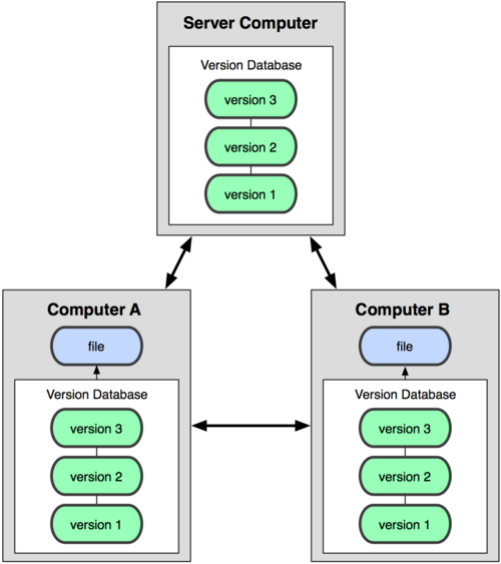
\includegraphics[width=0.4\textwidth]{images/local-vc.png}
    }
    \subfigure[集中化的版本控制系统]{
        \label{Fig.svn_model}
        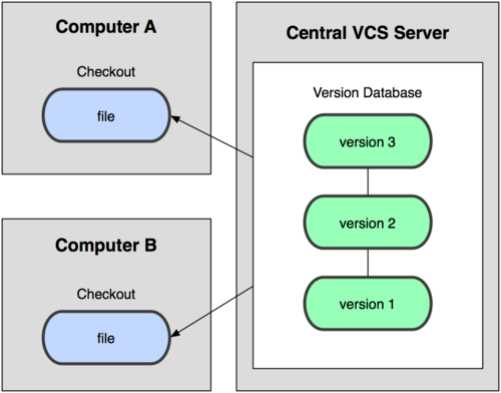
\includegraphics[width=0.5\textwidth]{images/svn-model.png}
    }

    \caption{本地代码管理和集中化的版本控制系统} %最终文档中希望显示的图片标题
    \label{Fig.svn_interge} %用于文内引用的标签
\end{figure}

这么做最显而易见的缺点是中央服务器的单点故障。若是宕机一小时,那么在这一小
时内,谁都无法提交更新,也就无法协同工作。如果中央服务器的磁盘发生故障,并且没做过备份或者备份得
不够及时的话,还会有丢失数据的风险。

% subsection SVN (end)

\subsection{Git} % (fold)
\label{sub:Git}

\subsubsection{Linus}


% subsection Git (end)



\newpage


\end{document}